\documentclass[border=5pt, multi, tikz]{standalone}
\usetikzlibrary{quotes,arrows.meta}

\definecolor{red}{rgb}{1,.5,.6}
\definecolor{blue}{rgb}{.5,.5,1}

\begin{document}

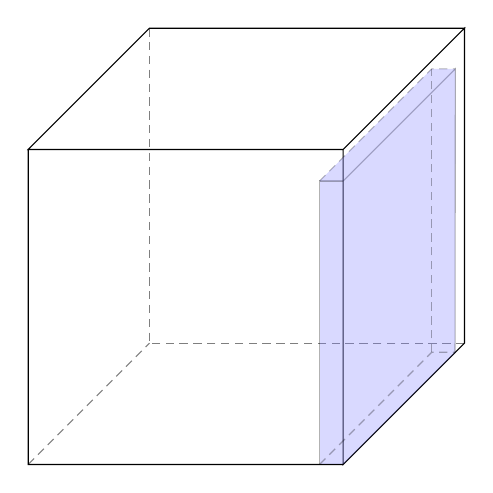
\begin{tikzpicture}
\draw [every edge/.append style={draw=black, densely dashed, opacity=.5}]
(0,0,0) coordinate (o) --
++(-4,0,0) coordinate (a) --
++(0,-4,0) coordinate (b) edge
coordinate [pos=1] (g) ++(0,0,-4) -- ++(4,0,0) coordinate (c) -- cycle
(o) -- ++(0,0,-4) coordinate (d) -- ++(0,-4,0) coordinate (e) edge (g) -- (c) -- cycle
(o) -- (a) -- ++(0,0,-4) coordinate (f) edge (g) -- (d) -- cycle;

\draw [fill=blue, opacity=.3] (0,-.4,0) -- (0,-.4,-3.7) -- (4,0,6.7) -- (0, -4, 0);

\draw [fill=blue, opacity=.3] (0,-.4,0) -- (-.3,-.4,0) -- (-.3,-4,0) -- (0,-4,0);

\draw[densely dashed, opacity=.3]  (-.3,-.4,0) -- (-.3,-.4,-3.7) -- (0,-.4,-3.7);

\fill[blue, opacity=.3]  (-.3,-.4,0) -- (-.3,-.4,-3.7) -- (0,-.4,-3.7) -- (0,-.4,0);

\draw[densely dashed, opacity=.3]  (-.3,-4,0) -- (-.3,-4,-3.7) -- (0,-4,-3.7);

\draw[densely dashed, opacity=.3]  (-.3,-4,-3.7) -- (-.3,-.4,-3.7);

\end{tikzpicture}
\end{document}
















